\chapter{Literature Review}
\label{literature_review}


As mentioned in the Introduction, it is only through the recent development of large open source datasets that statistical approaches to code related tasks have been available to machine learning researchers. 
As would be expected of any new and growing field, the range of attempted tasks is still expanding. 
Although as of writing no formal attempt has been made to translate fine grained elements of source code into their natural language descriptions, a great deal of relevant insight has been made in the related fields of source code summarization, variable naming, documentation generation, and code language modelling. 
These advances all highlight approaches to modelling the patterns and structure of code as language, whilst giving insight to methods of generating natural language from code, albeit at different levels of granularity.

In this review we summarise the current advances of these methods and how they relate to the task at hand.  

\section{Generating Language from Code}

One of the earliest statistical approaches to generating language from code comes from Movshovitz-Attias et al \cite{movshovitz-attias_natural_nodate}, who used ngrams and topic models to predict comments from JAVA source code.
By modelling the code and text as lexical ngrams in a mixed membership model, Moshovitz-Attias' model achieved a reasonable saving of characters to type on their comment completion task despite ignoring the semantic properties of the code.
This lexical approach to the language modelling of code was first established Hindle et al \cite{hindle_naturalness_nodate} who used a Kneser-Ney smoothed ngram model to demonstrate a lower cross entropy within corpora of JAVA and C code, than standard English corpora. This work had shown level of repetitiveness in code that was in concordance with work by Gabel and Su et al\cite{gabel_study_2010}, and was soon surpassed by ngram topic models that incorporated semantic information into the model, such as the models by Nyguyen et all \cite{nguyen_statistical_2013}.
Despite the simplistic treatment of the programming language, Moshovitz' comment generation demonstrated a positive start to the generation of language from code, and has opened up new tasks in the field.
%%% EXPLAIN N GRAM MODELS??


A popular such related task is that of code summarization, rather than comment prediction. This task involves taking large sections of code blocks, and summarising the meaning in natural language. It is very tied to the inverse problem of semantic parsing. 
An early approach to this work completely ignored the `naturalness' properties of code and surrounding comments, instead focusing on automatic rule-based summarization of the methods in consideration. This work, by Sridhara et al\cite{sridhara_[not_2010}, uses static analysis to find important subunits of code, and templates to produce English from these subunits.
Although this work produces text that accurately describes the functions in question, Sridhara notes the potential lack of transferrability to other languages, and lack of examples of exisiting comments to compare to, in the four java projects used in the study. Such a lack of data, indiciates a potential problem in the generalisability of the work.

Since then more statistical approaches have been used to attack the code summarization problem, utilizing much larger corpora of data. Iyer et al \cite{iyer_summarizing_2016} sourced a dataset of code snippets and descriptions from Stack Overflow, a popular programming website, comprising of 145,000 C\# examples and 41,000 SQL examles. 
They then apply a neural attentional model, CODE-NN, to this dataset, achieving the ``first learning techniques to construct completely new sentences from arbitrary code techniques''.   

This model combined a distributed representation of the code generated by an attention model, with an LSTM that operated on natural language tokens, to generate descriptions through a sequence of conditional distributions. 
Specifically this model calculated the probability of generating a length $l$
descriptive sequence through a product of conditional probabilities the previous $l-1$ tokens

$$P(\{n\}_1^l) = \prod_{i=1}^lp(n_i | n_1, ..., n_{i-1} ) $$

where each conditional probability was the proportional to a combination and non-linear transformation of the hidden state of the LSTM $\mathbf{h_i}$ and the attentional vector $\mathbf{t_i}$ at that point: 

$$\text p(n_i | n_1, ..., n_{i-1} ) \propto \mathbf{W}\text{tanh}(\mathbf{W_1h_i} + \mathbf{W_2t_i})$$

where $\mathbf{W} \in \mathbb{R}^{|N|\text{x} H}, \mathbf{W_1}$ and $\mathbf{W_2} \in \mathbb{R}^{H \text{x} H}$  and $ H$ is embedding dimensionality of words, $ N $ the vocabulary.\cite{iyer_summarizing_2016}
The calculation of LSTM $\mathbf{h_i}$ and the attentional vector $\mathbf{t_i}$ are described in the Background Section, while a visual representation of the model is preseted in Figure \ref{fig:Iyer}.

Although this This model performed exceptionally well on code summarization task, outperforming strong rival baselines, such as MOSES and SUMNN (cite) on the the BLEU-4 and METEOR metrics, it did this, without any consideration of the syntactical and semantic information of code. This indicated that a large part of the structure of code remains to be put to use by the model.
\begin{figure}[tb]
    \centering
    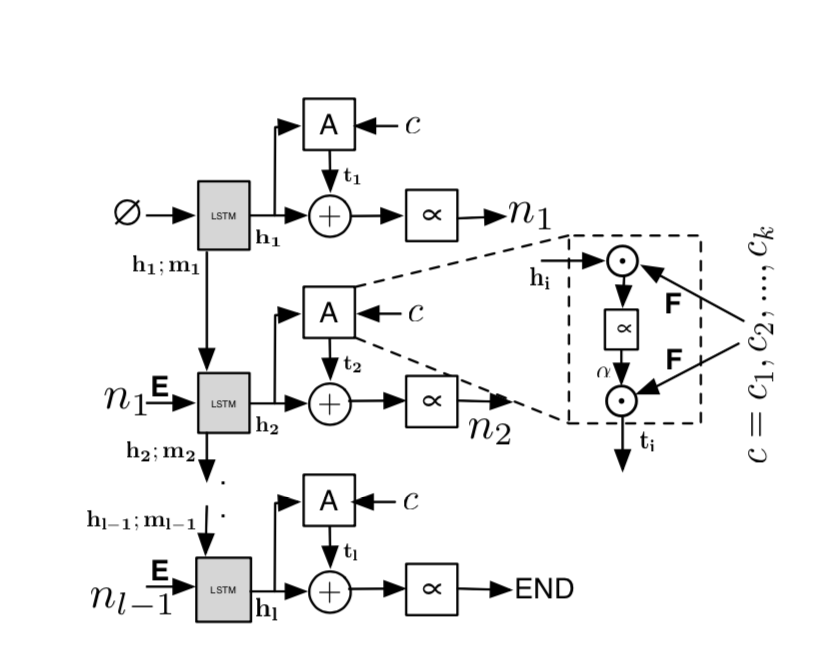
\includegraphics[width=0.5\linewidth]{ModelPics/Iyer_etal.png}
    \caption{Iyer et als Code NN, taken from \cite{iyer_summarizing_2016}}
    \label{fig:Iyer}
\end{figure}

Other models have shown promise in attention networks.




%  %drew inspiration from successes in recurrent neural networks in language modelling (CITE), and
% used of a neural attention model over source code tokens, combined with an LSTM accepting sequences of natural language tokens, to give distributions over the next token in the sequence.
% Specifically they modelled the probability of generating a length $l$
% descriptive sequence as a product of conditional probabilities the previous $l-1$ tokens
% % word sequence as a product of conditional probabilities over the next word, derived from the attentions and hidden states of the LSTM.
% % 
% $$P(\{n\}) = \prod_{i=1}^lp(n_i | n_1, ..., n_{i-1} ) $$

% where each conditional distribution was proportional to the combinations of the attentional representation and hidden state of the LSTM at that time.

% $$$$

% where 
% over the next word, whether the probabilities 

%  a distributional representation (PARA) of the source code would be calculated by an attention mechanism \cite{luong_effective_2015}, before being combined in addition with the hidden state $h_i$ of an LSTM (cite shmidthuber) and passed through a softmax layer to chose the next word in the description sequence. Each sequence 

 Summaries of Code changes - 


% Hindle's work  


% They built on work by Hindle, supported by SU
% This work ignores semantic information that could be benefitial. 

% This work specifically occurs at the level fo programming comments,

% A number of other pieces of work have since worked higher level summaries of code.
% Sridhara etc al templates
% Code NN summarization
% Related to semantic parsing - inverted. 
% Summaries of Code changes - 

% At the other end of the spectrum, code naming is treated a extremem summarization task, and has seen development.
% Other related tasks ro such include variable naming.

All